\chapter{Implementace}

Tato kapitola popisuje proces implementace navrhnutého řešení a popisuje použité nástroje.
Systém byl implementován podle návrhu v předchozí kapitole.
Dále jsou zde obsaženy vybrané ukázky kódu a výsledné podoby systému.

\section{Nástroje}

\subsection{Editor}

Pro vývoj kódu byl použit editor Visual Studio Code \cite{vscode}, který umožňuje snadnou integraci s verzovacím systémem
a podporuje množství typů souborů. Pomocí rozšiřujících doplňků je možné doplnit editor o pokročilé funkce či podporuj
dalších programovacích jazyků.

\subsection{Verzování}

K verzování projektu byl využit verzovací nástroj Git \cite{git}. Tento volně dostupný nástroj nabízí
neomezené distribuované verzování a je vhodný pro správu kódu.
Kód byl pomocí nástroje ukládán na webový server GitHub, který využívají i používané systémy TurnKey GNU/Linux
a LinuxGSM.

\subsection{Prostředí pro tvorbu obrazu}

Pro sestavení obrazu byl využit operační systém TKLDev \cite{tkldev}, provozovaný jako lokální virtuální stroj. Tento systém, spravovaný vývojáři TurnKey GNU/Linux,
je určen pro tvorbu nových obrazů této distribuce s přednastavenou aplikací. Umožňuje vytvářet obrazy ve formátech pro virtuální stroje a podporuje
také tvorbu obrazů určených k provozu u poskytovatelů cloudových služeb.

\section{Ukázky}

\subsection{Interaktivní výběr herního serveru}

Na obrázku \ref{fig:game-selection} je zobrazen interaktivní výběr herního serveru. Tento výběr je automaticky
k dispozici při prvním spuštění systému, pokud uživatel neurčil herní server pomocí inicializačního skriptu.

\begin{figure}[h]
    \centering
    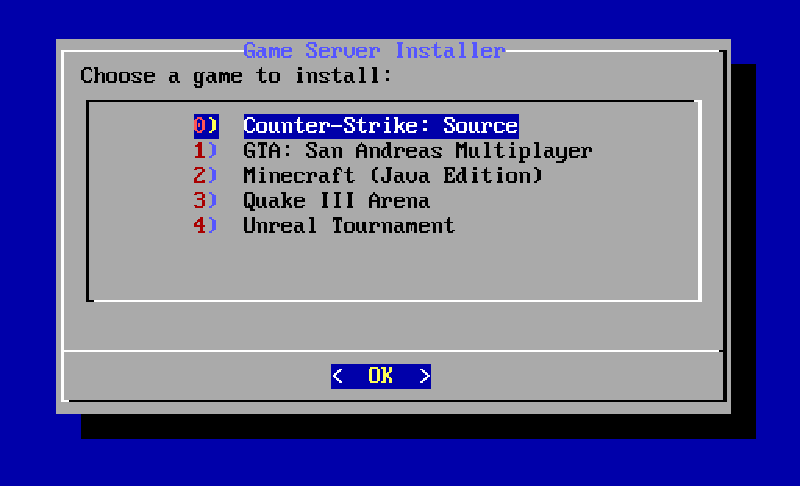
\includegraphics[width=1\linewidth]{chapters/images/game-selection.pdf}
    \caption{Interaktivní výběr hry při prvním spuštění}
    \label{fig:game-selection}
\end{figure}

\subsection{Automatický výběr herního serveru}

V případě plně automatického nasazení herního serveru je nutné použít inicializační skript, který před prvním spuštěním systému
zapíše do souboru \mintinline{shell}{/etc/inithooks.conf} potřebná data pro automatickou konfiguraci systému.
V ukázce \ref{code:init-script} je uveden inicializační skript, pomocí kterého dojde k instalaci herního serveru pro hru \mintinline{shell}{GTA: San Andreas Multiplayer}
včetně nastavení administrátora serveru.

\newpage

\begin{listing}[h!]
    \caption{Ukázkový inicializační skript}
    \label{code:init-script}
    \begin{minted}{shell}
#!/bin/bash

cat>/etc/inithooks.conf<<EOF
export ROOT_PASS=SecretRootPassword
export DB_PASS=SecretMysqlPassword
export APP_PASS=SecretGameuserPassword
export APP_EMAIL=admin@example.com
export HUB_APIKEY=SKIP
export SEC_UPDATES=FORCE

export GAME=samp
export GAME_RCON_PASS=GameserverAdminPassword
EOF
    \end{minted}
\end{listing}

\subsection{Přidání nové hry}

Ukázky \ref{code:game-props-script} a \ref{code:game-config-script} demonstrují přidání podpory pro nový herní server. Jedná se o dva skripty správce herních serverů,
které zavádějí podporu pro server hry \mintinline{shell}{Minecraft} a umožňují jeho minimální počáteční konfiguraci.
Skript \mintinline{shell}{game_properties.sh} zavádí proměnné, které jsou instalačním programem využity k identifikaci herního serveru.
Druhý skript poté umožňuje nastavit uživatelské jméno administrátora serveru pomocí předdefinované proměnné, případně interaktivně.

\begin{listing}[h]
    \caption{Skript \mintinline{shell}{game_properties.sh}}
    \label{code:game-props-script}
    \begin{minted}{shell}
GAME="mc"
GAME_LONG_NAME="Minecraft (Java Edition)"
    \end{minted}
\end{listing}

\begin{listing}[h]
    \caption{Skript \mintinline{shell}{post_install.sh}}
    \label{code:game-config-script}
    \begin{minted}{shell}
#!/bin/bash

# Set server admin
if [ -z "$GAME_ADMIN" ]; then
    read -p "Server admin username: " GAME_ADMIN || GAME_ADMIN=''
    echo
fi
run_as_user "echo \"$GAME_ADMIN\" > \"$GAMEDIR/serverfiles/ops.txt\""
    \end{minted}
\end{listing}

\section{Možnosti rozšíření}

Systém v současné době podporuje pouze čtyři herní tituly. Díky decentralizovanému návrhu
a osamostatnění části pro správu herních serverů od operačního systému je však možné doplňovat podporu
pro další herní servery bez zásahu do obrazu systému.

Některé herní servery vyžadují před spuštěním přihlášení k platformě Steam za účelem ověření zakoupení licence
pro jejich provoz. Tyto servery nejsou v současné chvíli systémem podporovány. V případě jejich podpory
by bylo nutné získat od uživatele jeho přihlašovací údaje, pomocí kterých by bylo možné licenci ověřit.

Systém je díky možnosti plně automatického spuštění vhodný i pro provoz v komerčním prostředí, vzhledem k aktuálnímu
množství podporovaných her ale není konkurenceschopný.

